% Bruselas
\newpage
%\thispagestyle{empty}
\begin{recipe}[source={La mami},
	portion={4 porciones},
	preparationtime={\unit[20]{Minutos}}
	]{Bruselas}
		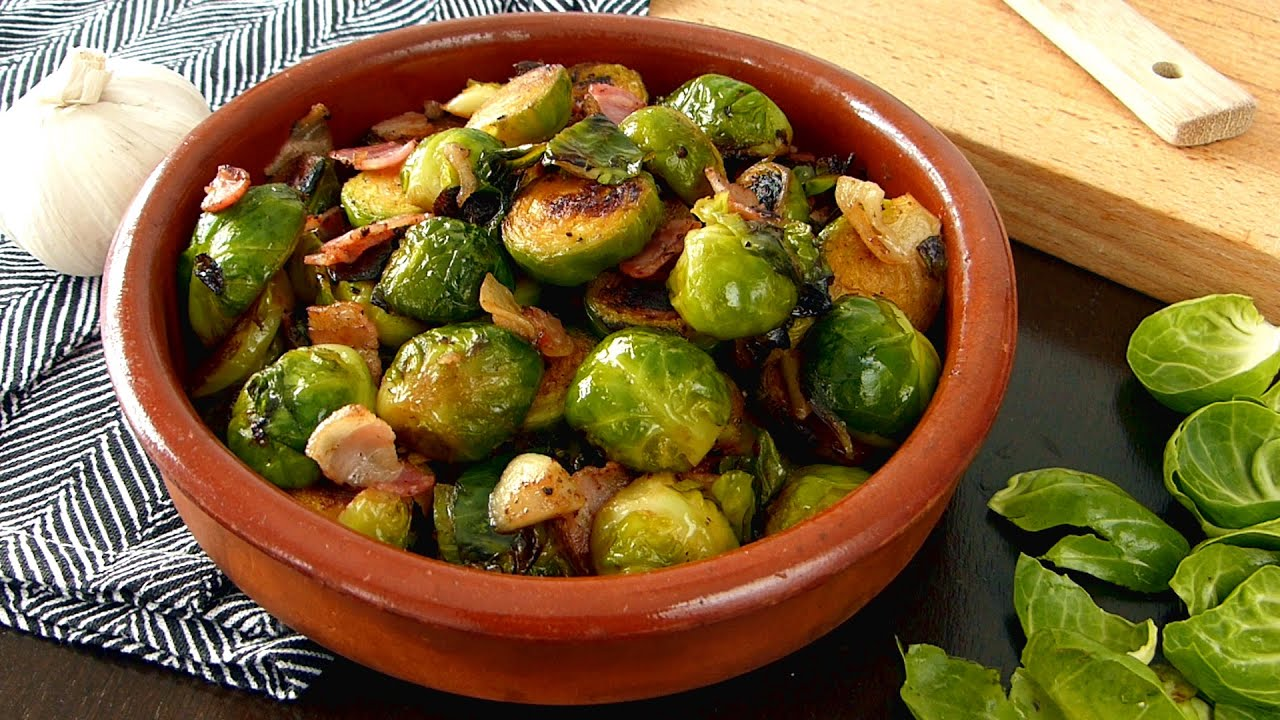
\includegraphics[width=0.25\textwidth]{bruselas}
	\introduction{
		Esta es una receta muy simple de realizar, es típico de las comidas chilenas
	}
	\ingredients{
		30 & bruselas \\
		& Sal
	}
	\preparation{
		\begin{enumerate}
			\item Lavar muy bien las bruselas, quitarles las hojas marchitas o cositas negras.
			\item En una olla llenar con agua hasta que cubra las bruselas, echar una cucharita de sal y aprovechar de lavar.
			\item Cambiar el agua, un poco de sal y al fuego fuerte hasta que hierva, luego bajar el fuego y dejar cocinar entre 15 y 20 minutos aproximadamente.
			\item Dejar enfriar, y servir.
		\end{enumerate}
	}
	\hint{
		Se puede acompañar con mayonesa al servir.
	}
\end{recipe}